\documentclass[12pt]{article}
\usepackage[letterpaper, margin=0.5in]{geometry}
\usepackage{newcent}

\usepackage{import}
\usepackage{graphics}
\usepackage{graphicx}


\begin{document}

\section{Learning to read sheet music}

So in music we use a music staff which is the 5 lines you see below.

{%
\parindent 0pt
\noindent
\ifx\preLilyPondExample \undefined
\else
  \expandafter\preLilyPondExample
\fi
\def\lilypondbook{}%
\input{b2/lily-bc2930a5-systems.tex}
\ifx\postLilyPondExample \undefined
\else
  \expandafter\postLilyPondExample
\fi
}

As you can see, for every increment higher on the staff the note name becomes the next letter. So if you start at \emph{e}, the space above it will be \emph{f}, the line above that will be \emph{g}.
And then once you reach the letter \emph{g} there are no note names after that so we wrap around to \emph{a} again.


{%
\parindent 0pt
\noindent
\ifx\preLilyPondExample \undefined
\else
  \expandafter\preLilyPondExample
\fi
\def\lilypondbook{}%
\input{fc/lily-c882d28a-systems.tex}
\ifx\postLilyPondExample \undefined
\else
  \expandafter\postLilyPondExample
\fi
}

The above is our mnemonic for remembering the values of the notes of each line. A note on the bottom line will be \emph{e}, the next will be \emph{g}, then \emph{b}, then \emph{d}, and finally the top line is \emph{f}. As the notes go up on the staff they get higher in pitch, and the lower you go the lower the pitch.


{%
\parindent 0pt
\noindent
\ifx\preLilyPondExample \undefined
\else
  \expandafter\preLilyPondExample
\fi
\def\lilypondbook{}%
\input{6b/lily-0dce5e10-systems.tex}
\ifx\postLilyPondExample \undefined
\else
  \expandafter\postLilyPondExample
\fi
}

We can remember this by saying, ``faces go in spaces.''

\section{Playing the Ukulele}
\subsection{The B-I-B-L-E}

\begin{figure}[ht!]
\centering
\includegraphics[height=3in]{ukulele.png}
\end{figure}

{%
\parindent 0pt
\noindent
\ifx\preLilyPondExample \undefined
\else
  \expandafter\preLilyPondExample
\fi
\def\lilypondbook{}%
\input{b8/lily-e366bee0-systems.tex}
\ifx\postLilyPondExample \undefined
\else
  \expandafter\postLilyPondExample
\fi
}

Try playing this on the ukulele. To do this, just pluck the top string, then the 2nd from the top, then the third and the fourth.

{%
\parindent 0pt
\noindent
\ifx\preLilyPondExample \undefined
\else
  \expandafter\preLilyPondExample
\fi
\def\lilypondbook{}%
\input{8a/lily-9057d928-systems.tex}
\ifx\postLilyPondExample \undefined
\else
  \expandafter\postLilyPondExample
\fi
}

Now figure out what notes these are and figure out which strings on your ukulele you're going to need to pluck to play them.

{%
\parindent 0pt
\noindent
\ifx\preLilyPondExample \undefined
\else
  \expandafter\preLilyPondExample
\fi
\def\lilypondbook{}%
\input{33/lily-6f9bebd3-systems.tex}
\ifx\postLilyPondExample \undefined
\else
  \expandafter\postLilyPondExample
\fi
}

Uh-oh, how do you play a \emph{d}? Well a \emph{d} is two half steps higher than a \emph{c}. So to play a \emph{d}, just put your finger on the second fret of your \emph{c string}. (If you put your finger on the first fret it's a \emph{c\#})

{%
\parindent 0pt
\noindent
\ifx\preLilyPondExample \undefined
\else
  \expandafter\preLilyPondExample
\fi
\def\lilypondbook{}%
\input{ba/lily-bee62701-systems.tex}
\ifx\postLilyPondExample \undefined
\else
  \expandafter\postLilyPondExample
\fi
}

There isn't an \emph{e\#} so the first fret of the \emph{e string} is an \emph{f}.
Here's all the possible notes, just pay attention to which have sharps.
\begin{quote}
a a\# b c c\# d d\# e f f\# g g\#
\end{quote}

So every fret you hold down takes you half a step higher than the name of the string. So 2 frets down on the \emph{a string} is a \emph{b}, and 3 frets down (3 half steps) is a \emph{c}.

{%
\parindent 0pt
\noindent
\ifx\preLilyPondExample \undefined
\else
  \expandafter\preLilyPondExample
\fi
\def\lilypondbook{}%
\input{f8/lily-b7e0244b-systems.tex}
\ifx\postLilyPondExample \undefined
\else
  \expandafter\postLilyPondExample
\fi
}


Don't use the \emph{c string} for the \emph{c}, it'll be an octave too low, you need to use the third fret on the \emph{a string}. What is an octave? Every time you're counting up on notes and you repeat that is a new octave. So
\begin{quote}
	c4 d4 e4 f4 g4 a4 b4 c5 d5 
\end{quote}
\emph{c4} is an octave lower than \emph{c5}. Notice that the octave numbers don't get higher until you reach \emph{c}, that's because \emph{c} is the start of every octave and not \emph{a} as you would think. Don't worry about the numbers for now, just pay attention to whether something is a low \emph{d} or a high \emph{d}. Octave means 8 because you have to count 8 notes to repeat a note if you keep going up or down (only the notes in a higher octave are higher sounding).

{%
\parindent 0pt
\noindent
\ifx\preLilyPondExample \undefined
\else
  \expandafter\preLilyPondExample
\fi
\def\lilypondbook{}%
\input{18/lily-6ab48ead-systems.tex}
\ifx\postLilyPondExample \undefined
\else
  \expandafter\postLilyPondExample
\fi
}

Practice playing this for a while. 

\subsection{Nothing But the Blood}

{%
\parindent 0pt
\noindent
\ifx\preLilyPondExample \undefined
\else
  \expandafter\preLilyPondExample
\fi
\def\lilypondbook{}%
\input{79/lily-ae96360d-systems.tex}
\ifx\postLilyPondExample \undefined
\else
  \expandafter\postLilyPondExample
\fi
}

For the most part we have been playing quarter notes,
but the notes that have holes in them are half notes and they are twice as long as a quarter note. But a dot next to a note makes it a half of its value longer, so a dotted quarter note would be a quarter note and an eighth note, and a dotted half note would be a half note and a quarter note (or 3 quarter notes). A note with a flag on it (or a bar if it's connected to another note) is an eighth note.

{%
\parindent 0pt
\noindent
\ifx\preLilyPondExample \undefined
\else
  \expandafter\preLilyPondExample
\fi
\def\lilypondbook{}%
\input{fe/lily-ed2939bf-systems.tex}
\ifx\postLilyPondExample \undefined
\else
  \expandafter\postLilyPondExample
\fi
}

Tap your foot at a steady rate to this song as you play. Hold each quarter note from when your foot hits the ground to when it hits the ground again. Hold a half note for 2 toe taps. For eighth notes do 2 of them in 1 tap.

{%
\parindent 0pt
\noindent
\ifx\preLilyPondExample \undefined
\else
  \expandafter\preLilyPondExample
\fi
\def\lilypondbook{}%
\input{c3/lily-a1af5d57-systems.tex}
\ifx\postLilyPondExample \undefined
\else
  \expandafter\postLilyPondExample
\fi
}

There are 4 quarter notes for every bar (or measure), so we can count them out like the above by saying what the start of the note we're on is.


{%
\parindent 0pt
\noindent
\ifx\preLilyPondExample \undefined
\else
  \expandafter\preLilyPondExample
\fi
\def\lilypondbook{}%
\input{5d/lily-08331c96-systems.tex}
\ifx\postLilyPondExample \undefined
\else
  \expandafter\postLilyPondExample
\fi
}

See how there's a swoopy line connecting the \emph{a} to the \emph{c} on snow? That's a slide. You play one note on a syllable and smoothly follow it up with a different note on the same syllable. If you see a note that with one of those curves connecting two notes that are the same pitch that is called a tie.

\end{document}
